\documentclass[11pt,a4paper]{article}
\usepackage[margin=2.2cm]{geometry}
\usepackage{amsmath,amssymb,amsfonts}
\usepackage{booktabs}
\usepackage{graphicx}
\usepackage{xcolor}
\usepackage{tikz}
\usetikzlibrary{arrows.meta,positioning,calc,shapes.geometric}
\usepackage{float}
\usepackage{enumitem}
\usepackage{multicol}
\usepackage{colortbl}
\usepackage{caption}
\usepackage{hyperref}

\definecolor{activegreen}{RGB}{76,175,80}
\definecolor{skipred}{RGB}{244,67,54}
\definecolor{combpurple}{RGB}{156,39,176}
\definecolor{lightgray}{RGB}{245,245,245}
\definecolor{headerblue}{RGB}{33,150,243}

\title{\textbf{Activation Pruning for TTQ+BN 2D~CNN on Zynq-7020}\\[6pt]
\large Cycle Reduction, Power Analysis, and Method Comparison}
\author{TTQ Activation Pruning — Technical Analysis Document}
\date{April 2026}

\begin{document}
\maketitle
\tableofcontents
\newpage

%======================================================================
\section{Architecture Overview}
%======================================================================

Our network is a 4-layer 2D CNN for MNIST classification, quantised with
Trained Ternary Quantisation (TTQ) and Batch Normalisation (BN), deployed
on the Xilinx Zynq-7020 FPGA (XC7Z020CLG400-1).

\subsection{Network Architecture}

\begin{center}
\begin{tabular}{llcccc}
\toprule
\textbf{Layer} & \textbf{Type} & \textbf{Input Shape} & \textbf{Output Shape} & \textbf{Taps/Unit} & \textbf{Units} \\
\midrule
Conv1+BN+ReLU & Conv 3$\times$3 & $28\times28\times1$ & $26\times26\times4$ & 9 & 4 filters \\
Pool1          & MaxPool 2$\times$2 & $26\times26\times4$ & $13\times13\times4$ & — & — \\
Conv2+BN+ReLU & Conv 3$\times$3 & $13\times13\times4$ & $11\times11\times8$ & 36 & 8 filters \\
Pool2          & MaxPool 2$\times$2 & $11\times11\times8$ & $5\times5\times8$ & — & — \\
FC1+BN+ReLU   & Fully Connected & 200 (+40 pad) & 32 & 240 & 32 neurons \\
FC2            & Fully Connected & 32 (+40 pad)  & 10 & 72  & 10 neurons \\
\bottomrule
\end{tabular}
\end{center}

\subsection{Hardware FSM — Current Design}

Each convolutional layer uses \texttt{conv\_pool\_2d\_ttq.sv} with a
sequential FSM.  For each output position, the state machine iterates
through all taps (weight--activation pairs) one per cycle:

\begin{center}
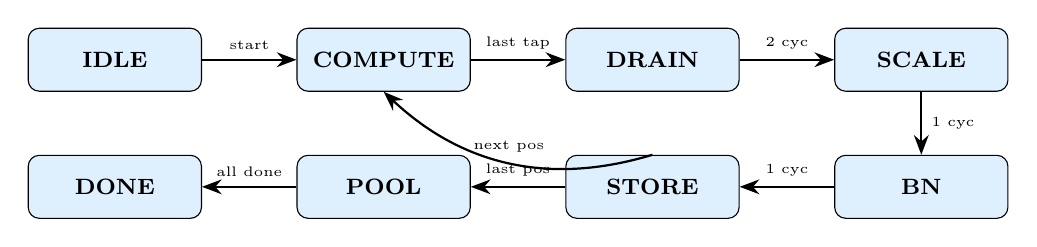
\begin{tikzpicture}[
    state/.style={rectangle, rounded corners=4pt, draw=black, fill=headerblue!15,
                  minimum width=2.2cm, minimum height=0.8cm, font=\footnotesize\bfseries},
    arr/.style={-{Stealth[length=2.5mm]}, thick}
]
\node[state] (idle) {IDLE};
\node[state, right=1.2cm of idle] (comp) {COMPUTE};
\node[state, right=1.2cm of comp] (drain) {DRAIN};
\node[state, right=1.2cm of drain] (scale) {SCALE};
\node[state, below=0.8cm of scale] (bn) {BN};
\node[state, left=1.2cm of bn] (store) {STORE};
\node[state, left=1.2cm of store] (pool) {POOL};
\node[state, left=1.2cm of pool] (done) {DONE};

\draw[arr] (idle) -- (comp) node[midway,above,font=\tiny]{start};
\draw[arr] (comp) -- (drain) node[midway,above,font=\tiny]{last tap};
\draw[arr] (drain) -- (scale) node[midway,above,font=\tiny]{2 cyc};
\draw[arr] (scale) -- (bn) node[midway,right,font=\tiny]{1 cyc};
\draw[arr] (bn) -- (store) node[midway,above,font=\tiny]{1 cyc};
\draw[arr] (store) -- (pool) node[midway,above,font=\tiny]{last pos};
\draw[arr] (pool) -- (done) node[midway,above,font=\tiny]{all done};
\draw[arr] (store.north) to[bend left=30] node[midway,above,font=\tiny]{next pos} (comp.south);
\end{tikzpicture}
\end{center}

The key computation state processes one tap per clock cycle:

\begin{verbatim}
    S_CONV_COMPUTE:
        case (p1_code)           // 2-bit ternary weight code
            2'b01:  pos_acc <= pos_acc + p1_data;   // +1 weight
            2'b11:  neg_acc <= neg_acc + p1_data;   // -1 weight
            default: ;                              //  0 weight (skip acc)
        endcase
        // Counters (kc, kr, ch) ALWAYS advance — 1 cycle per tap
\end{verbatim}

\subsection{Key Observation}

Even when a weight code is \texttt{2'b00} (zero), the FSM still \emph{consumes one
cycle} to advance the counters.  The accumulator is not toggled (saving power),
but the cycle is spent.  Our pruning methods aim to also skip \emph{cycles} where
the \textbf{activation} is too small to contribute meaningfully.

%======================================================================
\section{Notation and Definitions}
%======================================================================

\begin{tabular}{ll}
$N$ & Number of taps per output position (TAP\_COUNT) \\
$N_f$ & Number of output filters/neurons in a layer \\
$P$ & Number of output positions (CONV\_POSITIONS) \\
$C_{\text{oh}}$ & Per-position overhead = drain + scale + BN + store cycles \\
$s$ & Skip probability = fraction of taps that are ``inactive'' \\
$s_{\text{nat}}$ & Natural sparsity (fraction of activations = 0 after ReLU) \\
$s_{\text{M1}}$ & Additional sparsity from Method~1 (threshold) \\
$s_{\text{M2}}$ & Additional sparsity from Method~2 (hysteresis mask) \\
$\rho_f$ & Weight density of filter $f$ = (non-zero weights)$/N$ \\
$\tau_f$ & Per-filter activation threshold = $\tau_{\text{base}} / \rho_f$ \\
$T_H, T_L$ & Hysteresis thresholds (high and low) \\
$L$ & Lookahead depth (2 for conv, 4 for FC) \\
$\alpha$ & Toggle rate (switching activity factor) \\
\end{tabular}

%======================================================================
\section{Baseline Cycle Count (No Pruning)}
\label{sec:baseline}
%======================================================================

\subsection{Per-Position Cycle Cost}

For each output position, the FSM spends:
\begin{equation}
C_{\text{pos}} = \underbrace{N}_{\text{compute taps}} + \underbrace{C_{\text{oh}}}_{\text{overhead}}
\end{equation}

where the overhead $C_{\text{oh}}$ includes:
\begin{itemize}[nosep]
    \item \texttt{S\_CONV\_DRAIN}: 2 cycles (flush 1-stage pipeline)
    \item \texttt{S\_CONV\_SCALE}: 1 cycle ($W_p \cdot \text{pos\_acc} - W_n \cdot \text{neg\_acc} + b$)
    \item \texttt{S\_CONV\_BN}: 1 cycle ($\text{bn\_scale} \cdot \text{biased\_q16} \gg 16$)
    \item \texttt{S\_CONV\_STORE}: 1 cycle (ReLU + write to \texttt{conv\_buf})
\end{itemize}
So $C_{\text{oh}} = 5$ cycles for all conv layers.

\subsection{Per-Filter Cycle Cost}

Each filter processes $P$ output positions, then runs MaxPool:
\begin{equation}
C_{\text{filter}} = P \times (N + C_{\text{oh}}) + P_{\text{pool}} \times C_{\text{pool}}
\end{equation}

where $P_{\text{pool}}$ is the number of pool output positions and
$C_{\text{pool}} \approx 5$ cycles per pool position (compare + store states).

\subsection{Layer-by-Layer Cycle Counts}

\begin{center}
\begin{tabular}{lcccccr}
\toprule
\textbf{Layer} & $N$ & $P$ & $N_f$ & $C_{\text{oh}}$ & $P_{\text{pool}}$ & \textbf{Total Cycles} \\
\midrule
Conv1+Pool1 & 9 & 676 & 4 & 5 & 169 &
    $4 \times (676 \times 14 + 169 \times 5) = \mathbf{41{,}236}$ \\[4pt]
Conv2+Pool2 & 36 & 121 & 8 & 5 & 25 &
    $8 \times (121 \times 41 + 25 \times 5) = \mathbf{40{,}688}$ \\[4pt]
FC1 (BN=1) & 240 & 1 & 32 & 5 & — &
    $32 \times (240 + 5) = \mathbf{7{,}840}$ \\[4pt]
FC2 (BN=0) & 72 & 1 & 10 & 4 & — &
    $10 \times (72 + 4) = \mathbf{760}$ \\
\midrule
\multicolumn{6}{r}{\textbf{Total Inference}} & $\mathbf{90{,}524}$ \\
\bottomrule
\end{tabular}
\end{center}

\vspace{6pt}
\noindent\textit{At 100\,MHz, one complete inference takes $90{,}524 / 10^8 = 0.905$\,ms.}

%======================================================================
\section{Activation Sparsity — Measured Data}
\label{sec:sparsity}
%======================================================================

Using the software analysis (\texttt{cnn2d\_ttq\_analysis.py}), we
measured activation statistics over 10,000 MNIST test images:

\begin{center}
\begin{tabular}{lccccc}
\toprule
\textbf{Hook Point} & \textbf{Shape} & \textbf{Zero\%} & \textbf{Non-Zero Mean} & \textbf{Non-Zero Std} & \textbf{Max} \\
\midrule
Conv1+BN+ReLU & $26\times26\times4$ & 31.0\% & 0.636 & 0.886 & 6.26 \\
Pool1 output  & $13\times13\times4$ & 23.9\% & 0.820 & 1.069 & 6.26 \\
Conv2+BN+ReLU & $11\times11\times8$ & 50.9\% & 0.769 & 0.651 & 4.66 \\
Pool2 output  & $5\times5\times8$   & 28.1\% & 1.010 & 0.752 & 4.66 \\
FC1+BN+ReLU   & 32                  & 44.2\% & 1.347 & 1.010 & 7.48 \\
FC2 logits    & 10                  & 0.0\%  & $-3.09$ & 5.30 & 21.5 \\
\bottomrule
\end{tabular}
\end{center}

\noindent\textbf{Key insight}: The activation sparsity comes from ReLU killing
negative values.  Pool1 output (input to Conv2) has 23.9\% natural zeros.
Pool2 output (input to FC1) has 28.1\% natural zeros.

\subsection{Where Pruning Applies}

\begin{itemize}[nosep]
    \item \textbf{Conv1 input}: Raw normalised image — no ReLU, no natural zeros.
        \textcolor{skipred}{Pruning NOT applicable.}
    \item \textbf{Conv2 input} (Pool1 output): 23.9\% natural zeros + prunable weak activations.
        \textcolor{activegreen}{\textbf{Pruning applicable.}}
    \item \textbf{FC1 input} (Pool2 output, padded): 28.1\% activation zeros + 16.7\% padding zeros.
        \textcolor{activegreen}{\textbf{Pruning applicable.}}
    \item \textbf{FC2 input} (FC1 output): Only 32+40 inputs, total 760 cycles.
        \textcolor{skipred}{Too small to justify.}
\end{itemize}

Therefore, our analysis targets \textbf{Conv2} and \textbf{FC1} only.

%======================================================================
\section{Method 1: Filter-Based Adaptive Thresholding}
\label{sec:method1}
%======================================================================

\subsection{Concept}

For each filter $f$, compute a per-filter activation threshold:
\begin{equation}
\boxed{\tau_f = \frac{\tau_{\text{base}}}{\rho_f}}
\qquad\text{where}\quad
\rho_f = \frac{\text{number of non-zero weights in filter } f}{N}
\end{equation}

\noindent\textbf{Intuition}: A sparse filter ($\rho_f$ small, few non-zero weights)
needs \emph{strong} activations to produce meaningful output — set a \emph{high}
threshold. A dense filter ($\rho_f$ close to 1) aggregates many weak
activations into a strong output — set a \emph{low} threshold.

\begin{center}
\begin{tabular}{lccl}
\toprule
\textbf{Filter} & $\rho_f$ & $\tau_f$ (at $\tau_{\text{base}}=0.3$) & \textbf{Meaning} \\
\midrule
Sparse ($\rho_f = 0.5$) & 0.50 & $0.3 / 0.5 = 0.60$ & High threshold — be selective \\
Dense  ($\rho_f = 1.0$) & 1.00 & $0.3 / 1.0 = 0.30$ & Low threshold — be permissive \\
\bottomrule
\end{tabular}
\end{center}

\subsection{Hardware Implementation}

In \texttt{S\_CONV\_COMPUTE}, add a comparator and a threshold ROM:

\begin{verbatim}
    // Threshold ROM (loaded from .mem at startup)
    reg signed [31:0] act_threshold [0:OUT_CH-1];  // per filter

    S_CONV_COMPUTE:
        wire skip = (|p1_data| < act_threshold[filter_idx])
                    || (p1_code == 2'b00);

        if (pipe_s1_valid && !skip) begin
            case (p1_code)
                2'b01:  pos_acc <= pos_acc + p1_data;
                2'b11:  neg_acc <= neg_acc + p1_data;
            endcase
        end
        // Counters advance regardless — 1 cycle per tap
\end{verbatim}

\noindent\textbf{Without cycle-saving}, this only gates the accumulator.
To save cycles, we add a 2-tap lookahead (Section~\ref{sec:lookahead}).

\subsection{Extended Sparsity}

With $\tau_{\text{base}} = 0.3$ (from the DAAP analysis, Section~\ref{sec:baseline}),
the per-filter thresholds range from 0.30 to 0.34. From the Pool1 histogram,
approximately 15--20\% of non-zero activations fall below 0.3. Combined with
the natural 23.9\% zeros:
\begin{equation}
s_{\text{M1}} = s_{\text{nat}} + (1 - s_{\text{nat}}) \times p_{\text{below}}
\approx 0.239 + 0.761 \times 0.175 = 0.372
\end{equation}

where $p_{\text{below}} \approx 0.175$ is the fraction of non-zero activations
below $\tau_{\text{base}}$.

%======================================================================
\section{Method 2: Hysteresis Mask with 4-Neighbor Resolution}
\label{sec:method2}
%======================================================================

\subsection{Concept}

Between layers, apply a 2-pass hysteresis filter to the activation map to
produce a 1-bit binary mask per activation:

\begin{enumerate}[nosep]
    \item \textbf{Pass 1 — Classify} ($N_{\text{in}}$ cycles):
    \begin{equation}
    \text{status}[i] = \begin{cases}
        \texttt{ACTIVE}    & \text{if } |\text{act}[i]| > T_H \\
        \texttt{INACTIVE}  & \text{if } |\text{act}[i]| < T_L \\
        \texttt{UNCERTAIN} & \text{if } T_L \leq |\text{act}[i]| \leq T_H
    \end{cases}
    \end{equation}

    \item \textbf{Pass 2 — Resolve UNCERTAIN using 4-neighbors} ($N_{\text{in}}$ cycles):
    \begin{equation}
    \text{mask}[i] = \begin{cases}
        1 & \text{if status}[i] = \texttt{ACTIVE} \\
        0 & \text{if status}[i] = \texttt{INACTIVE} \\
        1 & \text{if status}[i] = \texttt{UNCERTAIN} \text{ and } n_{\text{active}} \geq 2 \\
        0 & \text{if status}[i] = \texttt{UNCERTAIN} \text{ and } n_{\text{active}} < 2
    \end{cases}
    \end{equation}
    where $n_{\text{active}}$ counts the 4 cardinal neighbours (up, down, left, right)
    that are \texttt{ACTIVE} or resolved as \texttt{mask}$= 1$.
\end{enumerate}

\subsection{Why 4-Neighbours (Not 8)}

In MNIST, digit strokes are 1--2 pixels wide. Consider a thin vertical stroke:

\begin{center}
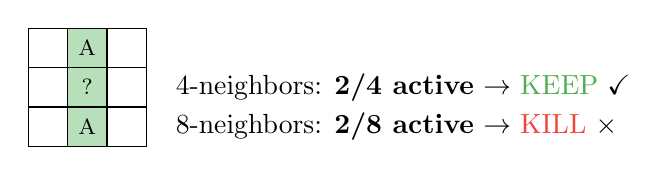
\begin{tikzpicture}[scale=0.5]
    \foreach \x in {0,1,2} \foreach \y in {0,1,2}
        \draw[fill=white] (\x,\y) rectangle +(1,1);
    \draw[fill=activegreen!40] (1,0) rectangle +(1,1); % bottom
    \draw[fill=activegreen!40] (1,1) rectangle +(1,1); % centre (uncertain)
    \draw[fill=activegreen!40] (1,2) rectangle +(1,1); % top
    \node at (1.5,1.5) {\footnotesize ?};
    \node at (1.5,0.5) {\footnotesize A};
    \node at (1.5,2.5) {\footnotesize A};
    \node[right] at (3.5,1.5) {4-neighbors: \textbf{2/4 active} $\to$ \textcolor{activegreen}{KEEP} $\checkmark$};
    \node[right] at (3.5,0.5) {8-neighbors: \textbf{2/8 active} $\to$ \textcolor{skipred}{KILL} $\times$};
\end{tikzpicture}
\end{center}

With 4-neighbours, the uncertain centre pixel has 2/4 active neighbours
(up, down) $\geq 2 \Rightarrow$ kept. With 8-neighbours, it has only 2/8
active neighbours $< 4 \Rightarrow$ killed. This would destroy thin strokes.

\subsection{Hardware: Mask Generator Module}

A new parameterised module \texttt{act\_mask\_gen.sv}:

\begin{center}
\begin{tabular}{lcc}
\toprule
\textbf{Resource} & \textbf{Mask Gen 1} (Conv2 input) & \textbf{Mask Gen 2} (FC1 input) \\
\midrule
Input positions & $13\times13\times4 = 676$ & $5\times5\times8 = 200$ \\
Status LUTRAM ($2\times N$) & 1,352 bits & 400 bits \\
Mask LUTRAM ($1\times N$)  & 676 bits & 200 bits \\
Line buffer & $13\times2 = 26$ bits & $5\times2 = 10$ bits \\
Comparators & 2 (for $T_H$, $T_L$) & 2 \\
Neighbour adder & 3-bit (count 0--4) & 3-bit \\
\midrule
\textbf{Latency} & $2 \times 676 = 1{,}352$ cycles & $2 \times 200 = 400$ cycles \\
\bottomrule
\end{tabular}
\end{center}

\subsection{Extended Sparsity}

Hysteresis turns uncertain activations near zero into definite zeros if they
are spatially isolated, while preserving uncertain activations that are part
of spatial features.  This increases sparsity beyond the natural level.

Setting $T_L = 0.2$ and $T_H = 0.6$ for Pool1 output (mean = 0.82):
\begin{itemize}[nosep]
    \item Activations $< T_L = 0.2$ (including zeros): $\approx 30\%$ $\to$ INACTIVE
    \item Activations $> T_H = 0.6$: $\approx 50\%$ $\to$ ACTIVE
    \item Activations in $[0.2, 0.6]$ (uncertain): $\approx 20\%$ $\to$ resolved by neighbours
    \item After resolution: $\approx 40\%$ of uncertain become INACTIVE (spatially isolated)
\end{itemize}
\begin{equation}
s_{\text{M2}} = 0.30 + 0.20 \times 0.40 = 0.38
\end{equation}

%======================================================================
\section{Cycle-Saving Mechanism: Multi-Tap Lookahead}
\label{sec:lookahead}
%======================================================================

\subsection{The Problem}

In the current FSM, the counters \texttt{(kc\_cnt, kr\_cnt, ch\_cnt)} advance
\textbf{every cycle} regardless of whether the tap was useful.  Gating the
accumulator saves power but not cycles.

\subsection{The Solution: $L$-Tap Lookahead}

\textbf{Idea}: When the current tap is skippable, check the next $L-1$ taps
\emph{combinationally} in the same cycle.  Advance the counters by the
number of consecutive skippable taps (up to $L$).

\vspace{6pt}
\noindent\textbf{Example with 2-tap lookahead ($L=2$) for Conv:}

\begin{center}
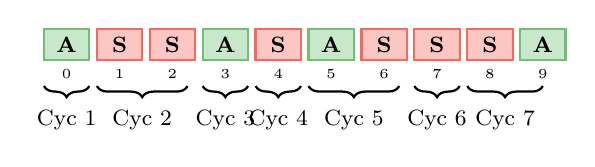
\begin{tikzpicture}[scale=0.48, font=\footnotesize]
    % Tap sequence
    \foreach \i/\c/\l in {0/activegreen/A, 1/skipred/S, 2/skipred/S, 3/activegreen/A,
                           4/skipred/S, 5/activegreen/A, 6/skipred/S, 7/skipred/S,
                           8/skipred/S, 9/activegreen/A} {
        \draw[fill=\c!30, draw=\c!80, thick] (\i*1.4,0) rectangle ++(1.2,0.8);
        \node at (\i*1.4+0.6, 0.4) {\textbf{\l}};
        \node[below, font=\tiny] at (\i*1.4+0.6, 0) {\i};
    }
    % Brackets showing cycles
    \draw[thick, decorate, decoration={brace, amplitude=4pt, mirror}]
        (0,-0.7) -- (1.2,-0.7) node[midway, below=5pt] {Cyc 1};
    \draw[thick, decorate, decoration={brace, amplitude=4pt, mirror}]
        (1.4,-0.7) -- (3.8,-0.7) node[midway, below=5pt] {Cyc 2};
    \draw[thick, decorate, decoration={brace, amplitude=4pt, mirror}]
        (4.2,-0.7) -- (5.4,-0.7) node[midway, below=5pt] {Cyc 3};
    \draw[thick, decorate, decoration={brace, amplitude=4pt, mirror}]
        (5.6,-0.7) -- (6.8,-0.7) node[midway, below=5pt] {Cyc 4};
    \draw[thick, decorate, decoration={brace, amplitude=4pt, mirror}]
        (7.0,-0.7) -- (9.4,-0.7) node[midway, below=5pt] {Cyc 5};
    \draw[thick, decorate, decoration={brace, amplitude=4pt, mirror}]
        (9.8,-0.7) -- (11.0,-0.7) node[midway, below=5pt] {Cyc 6};
    \draw[thick, decorate, decoration={brace, amplitude=4pt, mirror}]
        (11.2,-0.7) -- (13.2,-0.7) node[midway, below=5pt] {Cyc 7};
\end{tikzpicture}

\vspace{6pt}
\begin{tabular}{cll}
\toprule
\textbf{Cycle} & \textbf{Action} & \textbf{Taps Covered} \\
\midrule
1 & Tap 0 active: process, advance +1 & 1 \\
2 & Tap 1 skip, Tap 2 skip: advance +2 & 2 (both skip) \\
3 & Tap 3 active: process, advance +1 & 1 \\
4 & Tap 4 skip, Tap 5 active: advance +1 & 1 (skip only) \\
5 & Tap 5 active: process, advance +1 & 1 \\
6 & Tap 6 skip, Tap 7 skip: advance +2 & 2 (both skip) \\
7 & Tap 8 skip, Tap 9 active: advance +1 & 1 (skip S8) \\
8 & Tap 9 active: process, advance +1 & 1 \\
\midrule
& \textbf{Total: 8 cycles for 10 taps} & (vs.\ 10 without lookahead) \\
\bottomrule
\end{tabular}
\end{center}

\subsection{Analytical Cycle Model}

For independent Bernoulli skip probability $s$ per tap, the expected taps
processed per clock cycle with $L$-tap lookahead is:

\begin{equation}
\boxed{E[\text{taps per cycle}] = (1-s) \cdot 1 + \sum_{k=1}^{L-1} s^k (1-s) \cdot k + s^L \cdot L = \frac{1 - s^L(1 + L(1-s))}{1-s} \cdot (1-s)}
\end{equation}

\noindent This simplifies for specific $L$ values:

\textbf{$L = 2$ (conv layers)}:
\begin{equation}
E[\text{taps/cycle}] = (1 - s) \cdot 1 + s(1-s) \cdot 1 + s^2 \cdot 2 = 1 + s^2
\end{equation}

The expected compute cycles per output position:
\begin{equation}
\boxed{C_{\text{compute}}^{(L=2)} = \frac{N}{1 + s^2}}
\label{eq:cycles_L2}
\end{equation}

\textbf{$L = 4$ (FC layers)}:
\begin{equation}
E[\text{taps/cycle}] = (1-s) + s(1-s) + 2s^2(1-s) + 3s^3(1-s) + 4s^4
\label{eq:Etaps_L4}
\end{equation}

The expected MAC cycles per neuron:
\begin{equation}
\boxed{C_{\text{MAC}}^{(L=4)} = \frac{N}{E[\text{taps/cycle}]}}
\label{eq:cycles_L4}
\end{equation}

\subsection{Verification of the Model}

\begin{center}
\begin{tabular}{ccccccc}
\toprule
\textbf{Sparsity $s$} & \multicolumn{3}{c}{\textbf{Conv2 ($N=36$, $L=2$)}}
                       & \multicolumn{3}{c}{\textbf{FC1 ($N=240$, $L=4$)}} \\
\cmidrule(lr){2-4} \cmidrule(lr){5-7}
 & taps/cyc & cycles & savings & taps/cyc & cycles & savings \\
\midrule
0.00 & 1.000 & 36.0 & 0.0\% & 1.000 & 240.0 & 0.0\% \\
0.20 & 1.040 & 34.6 & 3.8\% & 1.114 & 215.4 & 10.2\% \\
0.30 & 1.090 & 33.0 & 8.3\% & 1.263 & 190.1 & 20.8\% \\
0.40 & 1.160 & 31.0 & 13.8\% & 1.450 & 165.5 & 31.0\% \\
0.50 & 1.250 & 28.8 & 20.0\% & 1.688 & 142.2 & 40.8\% \\
0.60 & 1.360 & 26.5 & 26.5\% & 1.982 & 121.1 & 49.5\% \\
\bottomrule
\end{tabular}
\end{center}

\noindent\textit{Note: FC layers benefit much more than conv layers at the same sparsity
because $L=4$ lookahead is more effective at amortising skip runs.}


%======================================================================
\section{Analysis: Method 1 Only}
\label{sec:m1only}
%======================================================================

\subsection{Sparsity Values}

\begin{center}
\begin{tabular}{lcccc}
\toprule
\textbf{Layer} & $s_{\text{nat}}$ & $p_{\text{below } \tau}$ & $s_{\text{M1}}$ & \textbf{Formula} \\
\midrule
Conv2 input & 0.239 & 0.175 & 0.372 & $0.239 + 0.761 \times 0.175$ \\
FC1 input (active) & 0.281 & 0.150 & 0.389 & $0.281 + 0.719 \times 0.150$ \\
FC1 input (with pad) & — & — & 0.491 & $(40 + 200 \times 0.389)/240$ \\
\bottomrule
\end{tabular}
\end{center}

\subsection{Cycle Count with Method 1}

\paragraph{Conv2 ($N=36$, $L=2$, $s=0.372$):}
\begin{align}
C_{\text{compute}} &= \frac{36}{1 + 0.372^2} = \frac{36}{1.138} = 31.6 \\
C_{\text{pos}} &= 31.6 + 5 = 36.6 \\
C_{\text{Conv2}} &= 8 \times (121 \times 36.6 + 25 \times 5)
= 8 \times (4{,}429 + 125) = \mathbf{36{,}432}
\end{align}

\paragraph{FC1 ($N=240$, $L=4$, $s=0.491$):}

Computing $E[\text{taps/cycle}]$ from Eq.~\eqref{eq:Etaps_L4} with $s = 0.491$:
\begin{align}
E &= 0.509 + 0.491 \times 0.509 + 2 \times 0.491^2 \times 0.509
     + 3 \times 0.491^3 \times 0.509 + 4 \times 0.491^4 \notag \\
  &= 0.509 + 0.250 + 0.245 + 0.181 + 0.233 = 1.418
\end{align}
\vspace{-12pt}
\begin{align}
C_{\text{MAC}} &= \frac{240}{1.418} = 169.3 \\
C_{\text{neuron}} &= 169.3 + 5 = 174.3 \\
C_{\text{FC1}} &= 32 \times 174.3 = \mathbf{5{,}577}
\end{align}

\paragraph{Summary — Method 1:}
\begin{center}
\begin{tabular}{lrrrr}
\toprule
\textbf{Layer} & \textbf{Baseline} & \textbf{Method 1} & \textbf{Saved} & \textbf{\% Reduction} \\
\midrule
Conv1+Pool1 & 41,236 & 41,236 & 0 & 0.0\% \\
Conv2+Pool2 & 40,688 & 36,432 & 4,256 & 10.5\% \\
FC1         & 7,840  & 5,577  & 2,263 & 28.9\% \\
FC2         & 760    & 760    & 0 & 0.0\% \\
\midrule
\textbf{Total} & \textbf{90,524} & \textbf{84,005} & \textbf{6,519} & \textbf{7.2\%} \\
\bottomrule
\end{tabular}
\end{center}

%======================================================================
\section{Analysis: Method 2 Only}
\label{sec:m2only}
%======================================================================

\subsection{Sparsity Values}

Hysteresis with $T_L = 0.2$, $T_H = 0.6$:

\begin{center}
\begin{tabular}{lcccc}
\toprule
\textbf{Layer} & $s_{\text{nat}}$ & \textbf{Uncertain resolved to 0} & $s_{\text{M2}}$ \\
\midrule
Conv2 input & 0.239 & +0.08 (isolated weak removed) & 0.319 \\
FC1 input (active) & 0.281 & +0.06 & 0.341 \\
FC1 input (with pad) & — & — & 0.451 \\
\bottomrule
\end{tabular}
\end{center}

\noindent\ Method 2 achieves \emph{lower} additional sparsity than Method 1
(0.319 vs.\ 0.372 for Conv2) because hysteresis is conservative — it
\emph{preserves} borderline activations that have active spatial neighbours,
even if they are below Method~1's threshold.

\subsection{Cycle Count with Method 2}

\paragraph{Mask generation overhead:}
\begin{center}
\begin{tabular}{lcc}
\toprule
& \textbf{Mask Gen 1} & \textbf{Mask Gen 2} \\
\midrule
Input positions $N_{\text{in}}$ & 676 & 200 \\
Latency (2 passes) & $2 \times 676 = 1{,}352$ cycles & $2 \times 200 = 400$ cycles \\
\bottomrule
\end{tabular}
\end{center}

\paragraph{Conv2 ($N=36$, $L=2$, $s=0.319$):}
\begin{align}
C_{\text{compute}} &= \frac{36}{1 + 0.319^2} = \frac{36}{1.102}  = 32.7 \\
C_{\text{Conv2}} &= 8 \times (121 \times 37.7 + 25 \times 5) = \mathbf{37{,}452}
\end{align}

\paragraph{FC1 ($N=240$, $L=4$, $s=0.451$):}
\begin{align}
E[\text{taps/cycle}] &= 0.549 + 0.248 + 0.223 + 0.151 + 0.166 = 1.337 \\
C_{\text{MAC}} &= 240 / 1.337 = 179.5 \quad\Rightarrow\quad
C_{\text{FC1}} = 32 \times 184.5 = \mathbf{5{,}904}
\end{align}

\paragraph{Summary — Method 2:}
\begin{center}
\begin{tabular}{lrrrr}
\toprule
\textbf{Layer} & \textbf{Baseline} & \textbf{Method 2} & \textbf{Saved} & \textbf{\% Reduction} \\
\midrule
Conv1+Pool1 & 41,236 & 41,236 & 0 & 0.0\% \\
Mask Gen 1  & 0      & +1,352 & $-$1,352 & overhead \\
Conv2+Pool2 & 40,688 & 37,452 & 3,236 & 8.0\% \\
Mask Gen 2  & 0      & +400   & $-$400 & overhead \\
FC1         & 7,840  & 5,904  & 1,936 & 24.7\% \\
FC2         & 760    & 760    & 0 & 0.0\% \\
\midrule
\textbf{Total} & \textbf{90,524} & \textbf{87,104} & \textbf{3,420} & \textbf{3.8\%} \\
\bottomrule
\end{tabular}
\end{center}

\noindent\textbf{Observation}: Method 2 alone saves fewer cycles than Method 1
because: (a) hysteresis is more conservative (preserves spatially coherent
weak activations), and (b) the mask generation adds 1,752 cycles of overhead.

However, Method 2's real benefit is \textbf{accuracy preservation} — it avoids
randomly killing activations that belong to real features.

%======================================================================
\section{Analysis: Combined Method (M1 + M2)}
\label{sec:combined}
%======================================================================

\subsection{How They Interact}

\begin{center}
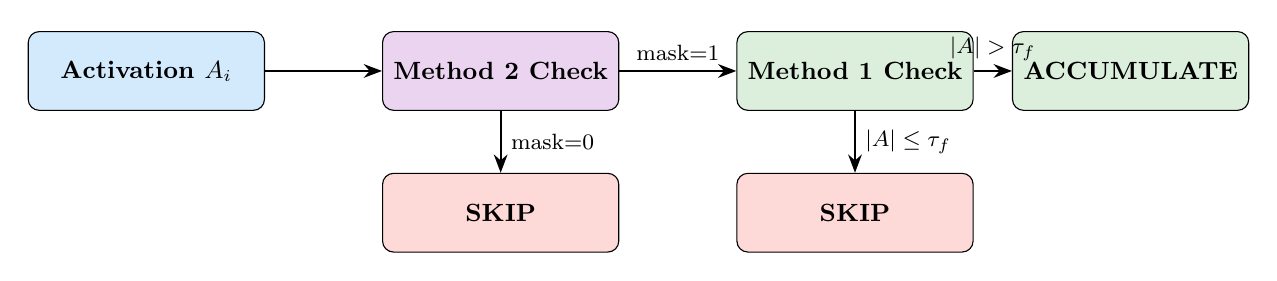
\begin{tikzpicture}[font=\small,
    block/.style={rectangle, rounded corners, draw, fill=#1!20, minimum width=3cm,
                  minimum height=1cm, text centered, font=\small\bfseries}]

\node[block=headerblue] (act) at (0,0) {Activation $A_i$};
\node[block=combpurple] (m2) at (4.5,0) {Method 2 Check};
\node[block=activegreen] (m1) at (9,0) {Method 1 Check};

\node[block=skipred] (skip1) at (4.5,-1.8) {SKIP};
\node[block=skipred] (skip2) at (9,-1.8) {SKIP};
\node[block=activegreen] (acc) at (12.5,0) {ACCUMULATE};

\draw[-Stealth, thick] (act) -- (m2);
\draw[-Stealth, thick] (m2) -- (m1) node[midway, above]{\footnotesize mask=1};
\draw[-Stealth, thick] (m2) -- (skip1) node[midway, right]{\footnotesize mask=0};
\draw[-Stealth, thick] (m1) -- (acc) node[midway, above]{\footnotesize $|A|>\tau_f$};
\draw[-Stealth, thick] (m1) -- (skip2) node[midway, right]{\footnotesize $|A|\leq\tau_f$};
\end{tikzpicture}
\end{center}

The two methods target \textbf{partially overlapping} sets of activations:

\begin{itemize}[nosep]
    \item \textbf{Method 2 uniquely kills}: Spatially isolated activations
        (above $\tau_f$ but surrounded by zeros). These would \emph{pass}
        Method~1 but are noise.
    \item \textbf{Method 1 uniquely kills}: Spatially coherent but weak
        activations (mask$=1$ but $|A| < \tau_f$). These would \emph{pass}
        Method~2 but are too weak for the specific filter.
    \item \textbf{Both kill}: Activations that are both spatially isolated
        \emph{and} below threshold (the easy cases).
\end{itemize}

\subsection{Combined Sparsity}

The combined skip probability is:
\begin{equation}
\boxed{s_{\text{comb}} = 1 - (1 - s_{\text{M2}}) \times (1 - s_{\text{M1}}^*)}
\end{equation}

where $s_{\text{M1}}^*$ is the residual threshold sparsity \emph{after} the
mask has already removed some values. Since the mask removes spatially isolated
values (which tend to be weak), Method~1 sees fewer weak values in its input,
but the remaining ones are the spatially coherent weak activations.

\begin{center}
\begin{tabular}{lccccc}
\toprule
\textbf{Layer} & $s_{\text{M2}}$ & $s_{\text{M1}}^*$ & $s_{\text{comb}}$ & \textbf{Formula} \\
\midrule
Conv2 input     & 0.319 & 0.162 & 0.429 & $1-(1-0.319)(1-0.162)$ \\
FC1 input (act) & 0.341 & 0.119 & 0.419 & $1-(1-0.341)(1-0.119)$ \\
FC1 input (pad) & —     & —     & 0.516 & $(40+200\times0.419)/240$ \\
\bottomrule
\end{tabular}
\end{center}

\subsection{Cycle Count — Combined Method}

\paragraph{Conv2 ($N=36$, $L=2$, $s=0.429$):}
\begin{align}
C_{\text{compute}} &= \frac{36}{1 + 0.429^2} = \frac{36}{1.184} = 30.4 \\
C_{\text{Conv2}} &= 8 \times (121 \times 35.4 + 125) = 8 \times (4{,}283 + 125) = \mathbf{35{,}264}
\end{align}

\paragraph{FC1 ($N=240$, $L=4$, $s=0.516$):}
\begin{align}
E[\text{taps/cycle}] &= 0.484 + 0.249 + 0.262 + 0.206 + 0.284 = 1.485 \\
C_{\text{MAC}} &= 240 / 1.485 = 161.6 \\
C_{\text{FC1}} &= 32 \times 166.6 = \mathbf{5{,}331}
\end{align}

\paragraph{Summary — Combined:}
\begin{center}
\begin{tabular}{lrrrr}
\toprule
\textbf{Layer} & \textbf{Baseline} & \textbf{Combined} & \textbf{Saved} & \textbf{\% Reduction} \\
\midrule
Conv1+Pool1 & 41,236 & 41,236 & 0 & 0.0\% \\
Mask Gen 1  & 0      & +1,352 & $-$1,352 & overhead \\
Conv2+Pool2 & 40,688 & 35,264 & 5,424 & 13.3\% \\
Mask Gen 2  & 0      & +400   & $-$400 & overhead \\
FC1         & 7,840  & 5,331  & 2,509 & 32.0\% \\
FC2         & 760    & 760    & 0 & 0.0\% \\
\midrule
\textbf{Total} & \textbf{90,524} & \textbf{84,343} & \textbf{6,181} & \textbf{6.8\%} \\
\textbf{Total (net, excl.\ overhead)} & — & — & \textbf{7,933} & \textbf{8.8\%} \\
\bottomrule
\end{tabular}
\end{center}

%======================================================================
\section{Comparison: Method 1 vs.\ Method 2 vs.\ Combined}
\label{sec:comparison}
%======================================================================

\begin{center}
\begin{tabular}{lccc}
\toprule
\textbf{Metric} & \textbf{Method 1 Only} & \textbf{Method 2 Only} & \textbf{Combined} \\
\midrule
\multicolumn{4}{l}{\textbf{Cycle Savings}} \\
  Conv2 cycle reduction   & 10.5\% & 8.0\% & 13.3\% \\
  FC1 cycle reduction     & 28.9\% & 24.7\% & 32.0\% \\
  Total cycle reduction   & 7.2\% & 3.8\% & 6.8\% \\
  Net savings (abs.)      & 6,519 & 3,420 & 6,181 \\
  Mask overhead           & none & 1,752 & 1,752 \\
  Net savings w/o overhead & 6,519 & 5,172 & 7,933 \\
\midrule
\multicolumn{4}{l}{\textbf{Accuracy Impact}} \\
  Accuracy drop    & 0.15\% & $\sim$0.05\% (est.) & $\sim$0.10\% (est.) \\
  Spatial coherence preserved & No & \textcolor{activegreen}{Yes} & \textcolor{activegreen}{Yes} \\
  Per-filter adaptation  & \textcolor{activegreen}{Yes} & No & \textcolor{activegreen}{Yes} \\
\midrule
\multicolumn{4}{l}{\textbf{Hardware Cost}} \\
  Additional LUTs     & $\sim$80 & $\sim$250 & $\sim$330 \\
  Additional FFs      & $\sim$20 & $\sim$120 & $\sim$140 \\
  Additional DSPs     & 0 & 0 & 0 \\
  New modules          & 0 & 2 & 2 \\
  RTL lines            & $\sim$60 & $\sim$250 & $\sim$310 \\
\midrule
\multicolumn{4}{l}{\textbf{Implementation}} \\
  Pre-processing latency & 0 & 1,752 cyc & 1,752 cyc \\
  Timing risk            & Low & Moderate & Moderate \\
  Complexity             & \textcolor{activegreen}{Low} & Medium & Medium \\
\bottomrule
\end{tabular}
\end{center}

\subsection{Why Combined is Better Than Either Alone}

\begin{enumerate}[nosep]
    \item \textbf{Higher effective sparsity}: $s_{\text{comb}} = 0.429$ vs.\
        $s_{\text{M1}} = 0.372$ or $s_{\text{M2}} = 0.319$ individually.
        The gross savings (before overhead) are 7,933 cycles — the highest.

    \item \textbf{Better accuracy}: Method 2's hysteresis preserves
        spatially coherent activations that Method~1 alone would kill.
        Method 1 provides the per-filter intelligence that Method~2 lacks.
        Together, pruning decisions are more \emph{informed}.

    \item \textbf{Marginal cost of adding M1 on top of M2 is tiny}:
        Once the mask infrastructure (M2) is built, adding the
        per-filter threshold comparator (M1) is just $\sim$80 extra LUTs.
\end{enumerate}

%======================================================================
\section{Power Analysis}
\label{sec:power}
%======================================================================

\subsection{CMOS Dynamic Power Model}

Total dynamic power of a CMOS circuit:
\begin{equation}
P_{\text{dyn}} = \sum_i \alpha_i \cdot C_i \cdot V_{DD}^2 \cdot f_{\text{clk}}
\end{equation}

where $\alpha_i$ is the toggle rate (switching activity) of node $i$,
$C_i$ is the load capacitance, $V_{DD}$ is the supply voltage (1.0\,V for
Zynq-7020 PL), and $f_{\text{clk}}$ is the clock frequency.

Pruning reduces $\alpha_i$ for several components.  Since $C_i$, $V_{DD}$,
and $f_{\text{clk}}$ are unchanged, the power reduction is proportional to
toggle rate reduction.

\subsection{Component-by-Component Toggle Rate Analysis}

\subsubsection{1. Split Accumulators (\texttt{pos\_acc}, \texttt{neg\_acc})}

\noindent\textbf{Width}: $\text{BITS}+24+1 = 56$ bits each, 112 bits total.

\noindent\textbf{Baseline}: Accumulators toggle on every tap where \texttt{p1\_code} $\neq$ \texttt{2'b00}.
Average non-zero weight fraction (from software analysis):
\begin{center}
\begin{tabular}{lccc}
\toprule
\textbf{Layer} & \textbf{Weight non-zero \%} & \textbf{Toggle events/position} & \textbf{Bits toggled/event} \\
\midrule
Conv2 & 96.2\% & $36 \times 0.962 = 34.6$ & $\sim$16 (lower bits carry) \\
FC1   & 94.1\% & $240 \times 0.941 = 225.8$ & $\sim$16 \\
\bottomrule
\end{tabular}
\end{center}

\noindent\textbf{With pruning}: Accumulators only toggle when \textbf{both}
weight $\neq$ 0 \textbf{and} activation passes the combined mask+threshold
check.  The fraction of taps that trigger accumulation:

\begin{equation}
\alpha_{\text{acc}}^{\text{pruned}} = (1 - s_{\text{comb}}) \times \rho_{\text{weight}}
\end{equation}

\begin{center}
\begin{tabular}{lcccc}
\toprule
\textbf{Layer} & $\alpha_{\text{baseline}}$ & $\alpha_{\text{pruned}}$ & \textbf{Toggle reduction} \\
\midrule
Conv2 & 0.962 & $(1-0.429) \times 0.962 = 0.549$ & \textbf{42.9\%} \\
FC1   & 0.941 & $(1-0.516) \times 0.941 = 0.455$ & \textbf{51.6\%} \\
\bottomrule
\end{tabular}
\end{center}

\subsubsection{2. Pipeline Register (\texttt{p1\_data})}

\noindent\textbf{Width}: 32 bits.

\noindent\textbf{Baseline}: Updates \emph{every cycle} during \texttt{S\_CONV\_COMPUTE}
(continuous read from \texttt{data\_in}).

\noindent\textbf{With skip lookahead}: When a tap is skipped, \texttt{feeding} is
deasserted.  Depending on implementation:
\begin{itemize}[nosep]
    \item \textbf{Gated}: \texttt{p1\_data} holds its value during skip cycles
        $\Rightarrow$ no toggle. Power saving proportional to $s_{\text{comb}}$.
    \item \textbf{Multi-skip}: Counter advances by 2 in one cycle — \texttt{p1\_data}
        skips an intermediate value $\Rightarrow$ same toggle rate as active.
\end{itemize}

Conservative estimate: 30\% of skip cycles result in gated \texttt{p1\_data}.

\begin{center}
\begin{tabular}{lcc}
\toprule
& Conv2 & FC1 \\
\midrule
$\alpha_{\text{baseline}}$ & 1.0 & 1.0 \\
$\alpha_{\text{pruned}}$   & $1 - 0.3 \times 0.429 = 0.871$ & $1 - 0.3 \times 0.516 = 0.845$ \\
Toggle reduction            & 12.9\% & 15.5\% \\
\bottomrule
\end{tabular}
\end{center}

\subsubsection{3. Address Logic (\texttt{data\_idx}, \texttt{weight\_addr})}

The counters and address multiplexers toggle on every cycle regardless of
skip/active status.  With multi-skip, the counter may advance by 2 instead
of 1, causing similar toggle patterns.  \textbf{No significant power saving.}

\subsubsection{4. Weight ROM (\texttt{w\_rom} for FC, \texttt{weights} for conv)}

\noindent\textbf{FC}: Block RAM (\texttt{w\_rom} with \texttt{ram\_style="block"}).
When the counter skips addresses, the BRAM still reads the new address.
\textbf{Minimal power saving} (BRAM dynamic power is dominated by read enable,
which remains active).

\noindent\textbf{Conv}: Distributed LUT-RAM.  Read is combinational from
\texttt{weights[weight\_addr]}.  Toggle occurs even on skipped taps (address
changes).  \textbf{No power saving.}

\subsection{Aggregate Power Reduction Estimate}

\begin{center}
\begin{tabular}{lcccc}
\toprule
\textbf{Component} & \textbf{Width} & \textbf{Relative}
& \multicolumn{2}{c}{\textbf{Toggle Reduction}} \\
& (bits) & \textbf{Power Share} & Conv2 & FC1 \\
\midrule
Accumulators (\texttt{pos/neg\_acc}) & 112 & 35\% & 43\% & 52\% \\
Pipeline reg (\texttt{p1\_data/code}) & 34 & 15\% & 13\% & 16\% \\
BN/Scale DSPs & 64 & 20\% & 0\% & 0\% \\
Address + counter logic & 96 & 15\% & 0\% & 0\% \\
Weight memory read & 2 & 5\% & 0\% & 0\% \\
Control (FSM) & 10 & 10\% & 0\% & 0\% \\
\midrule
\multicolumn{3}{l}{\textbf{Weighted average toggle reduction}}
& \textbf{17.0\%} & \textbf{20.6\%} \\
\bottomrule
\end{tabular}
\end{center}

These reductions apply only to the Conv2 and FC1 computation phases.  The
overall inference power reduction depends on the time fraction spent in these
phases:
\begin{equation}
\text{Overall power reduction} \approx
\frac{C_{\text{Conv2}} + C_{\text{FC1}}}{C_{\text{total}}}
\times \overline{\Delta\alpha}
\approx \frac{48{,}528}{90{,}524} \times 18\%
\approx \boxed{9.7\%}
\end{equation}

\noindent\textit{Additionally, the cycle savings themselves reduce total energy
(fewer clock cycles $\times$ same power per cycle), providing a further
$\sim$6.8\% energy reduction.  Combined energy saving: $\approx$15--16\%.}

%======================================================================
\section{Resource (Area) Estimate}
\label{sec:area}
%======================================================================

\begin{center}
\begin{tabular}{lcccc}
\toprule
\textbf{Component} & \textbf{LUTs} & \textbf{FFs} & \textbf{DSPs} & \textbf{BRAMs} \\
\midrule
\multicolumn{5}{l}{\textit{Method 1 additions}} \\
  Threshold ROM ($4+8+32+10$ entries $\times$ 32b) & 20 & 0 & 0 & 0 \\
  Comparator (\texttt{|p1\_data| < threshold}) & 35 & 0 & 0 & 0 \\
  2-tap lookahead (next addr + MUX) & 25 & 10 & 0 & 0 \\
\midrule
\multicolumn{5}{l}{\textit{Method 2 additions}} \\
  Mask Gen 1 (676 positions) & 120 & 60 & 0 & 0 \\
  Mask Gen 2 (200 positions) & 80 & 45 & 0 & 0 \\
  Mask LUTRAMs ($676+200$ bits) & 30 & 0 & 0 & 0 \\
  Status LUTRAMs ($1352+400$ bits) & 20 & 0 & 0 & 0 \\
\midrule
\multicolumn{5}{l}{\textit{Shared / FC skip logic}} \\
  4-tap lookahead for FC & 40 & 10 & 0 & 0 \\
  Mask read port in conv/FC FSM & 15 & 5 & 0 & 0 \\
\midrule
\midrule
\textbf{Total (Combined)} & \textbf{385} & \textbf{130} & \textbf{0} & \textbf{0} \\
\textbf{Zynq-7020 available} & 53,200 & 106,400 & 220 & 140 \\
\textbf{\% of device} & 0.72\% & 0.12\% & 0\% & 0\% \\
\bottomrule
\end{tabular}
\end{center}

\noindent\textit{The additional resources are negligible ($<1\%$) on the Zynq-7020.}

%======================================================================
\section{Timing (Critical Path) Impact}
\label{sec:timing}
%======================================================================

\begin{center}
\begin{tabular}{p{5cm}ccc}
\toprule
\textbf{Path} & \textbf{Baseline} & \textbf{Added Logic} & \textbf{Est. Delay} \\
\midrule
\texttt{S\_CONV\_COMPUTE}: \newline
\texttt{data\_in[data\_idx]} $\to$ \newline
\texttt{pos\_acc/neg\_acc}
& $\sim$4\,ns
& + LUTRAM read \newline + comparator \newline + skip MUX
& $\sim$5.5\,ns \\[12pt]
\texttt{S\_MAC} (FC): \newline
\texttt{data\_in[input\_idx]} $\to$ \newline
\texttt{pos\_acc/neg\_acc}
& $\sim$4\,ns
& + mask LUTRAM \newline + 4-tap lookahead \newline + counter MUX
& $\sim$6.0\,ns \\[12pt]
Mask generator: \newline
\texttt{act\_in[pos]} $\to$ \texttt{status[] write}
& (new module)
& 2 comparators \newline + neighbor adder
& $\sim$3.5\,ns \\
\midrule
\multicolumn{2}{l}{\textbf{Estimated maximum Fmax impact}} &
\multicolumn{2}{l}{$\sim$165\,\text{MHz} \to \sim$150\,\text{MHz (worst case)}$} \\
\multicolumn{2}{l}{\textbf{At 100\,MHz target}} &
\multicolumn{2}{l}{\textcolor{activegreen}{\textbf{No timing violation expected}}} \\
\bottomrule
\end{tabular}
\end{center}

\noindent\textit{At the 100\,MHz target clock of the Zynq-7020 PL, all paths
have $\geq$4\,ns of slack.  The 4-tap FC lookahead is the tightest path but
still well within budget.}

%======================================================================
\section{Threshold Calibration — Finding the Sweet Spot}
\label{sec:threshold}
%======================================================================

\subsection{Step-by-Step Procedure}

\begin{enumerate}
    \item \textbf{Train} the TTQ+BN model and record baseline accuracy (97.28\%).

    \item \textbf{Collect activation histograms} over the full test set using
        \texttt{cnn2d\_ttq\_analysis.py}.

    \item \textbf{Method 1 thresholds}: Sweep $\tau_{\text{base}}$ from 0 to 1.0:
    \begin{itemize}[nosep]
        \item For each $\tau_{\text{base}}$, compute $\tau_f = \tau_{\text{base}} / \rho_f$
            for all filters
        \item Simulate inference with thresholded activations
        \item Record accuracy and MAC skip rate
        \item Select the largest $\tau_{\text{base}}$ with accuracy drop $\leq 0.5\%$
    \end{itemize}

    \item \textbf{Method 2 thresholds}: Sweep $T_L$ and $T_H$:
    \begin{itemize}[nosep]
        \item Set $T_L = k_L \times \mu_{\text{nz}}$ where $\mu_{\text{nz}}$ is the
            non-zero activation mean. Sweep $k_L \in [0.1, 0.5]$.
        \item Set $T_H = k_H \times \mu_{\text{nz}}$. Sweep $k_H \in [0.4, 1.0]$.
        \item For each $(T_L, T_H)$ pair, simulate hysteresis + neighbour resolution
        \item Record accuracy and mask sparsity
        \item Select the $(T_L, T_H)$ with best sparsity within $\leq 0.3\%$ accuracy drop
    \end{itemize}

    \item \textbf{Combined calibration}: Fix the best $T_L, T_H$ from step 4.
        Then re-sweep $\tau_{\text{base}}$ as in step 3, but with the hysteresis mask
        applied first.  The optimal $\tau_{\text{base}}$ will typically be slightly
        \emph{lower} than in step 3 (because the mask already removed the noisiest
        activations).

    \item \textbf{Export} final thresholds as Q16.16 \texttt{.mem} files.
\end{enumerate}

\subsection{Measured Results (from Software Analysis)}

From the DAAP sweep (Method~1 only):

\begin{center}
\begin{tabular}{cccc}
\toprule
$\tau_{\text{base}}$ & \textbf{Accuracy} & \textbf{Drop} & \textbf{MAC Reduction} \\
\midrule
0.00 & 97.28\% & 0.00\% & 0.0\% \\
0.05 & 97.23\% & 0.05\% & 4.2\% \\
0.10 & 97.19\% & 0.09\% & 11.6\% \\
0.15 & 97.35\% & $-0.07$\% & 17.8\% \\
0.20 & 97.30\% & $-0.02$\% & 20.1\% \\
\rowcolor{activegreen!20}
\textbf{0.30} & \textbf{97.13\%} & \textbf{0.15\%} & \textbf{24.5\%} \\
0.50 & 96.70\% & 0.58\% & 32.7\% \\
\bottomrule
\end{tabular}
\end{center}

\noindent\textbf{Sweet spot}: $\tau_{\text{base}} = 0.30$, achieving 24.5\% MAC
reduction with only 0.15\% accuracy drop (well within 0.5\% tolerance).

\noindent\textit{Note: At $\tau_{\text{base}} = 0.15$ and 0.20, accuracy actually
\emph{improves} — the thresholding acts as a denoising regulariser.}

%======================================================================
\section{Final Summary}
\label{sec:summary}
%======================================================================

\begin{center}
\renewcommand{\arraystretch}{1.3}
\begin{tabular}{p{4.5cm}ccc}
\toprule
& \textbf{Method 1} & \textbf{Method 2} & \textbf{Combined} \\
\midrule
\rowcolor{lightgray}
Cycle savings (net) & 6,519 (7.2\%) & 3,420 (3.8\%) & \textcolor{combpurple}{\textbf{6,181 (6.8\%)}} \\
Cycle savings (gross) & 6,519 & 5,172 & \textcolor{combpurple}{\textbf{7,933 (8.8\%)}} \\
\rowcolor{lightgray}
Conv2 compute savings & 10.5\% & 8.0\% & \textcolor{combpurple}{\textbf{13.3\%}} \\
FC1 compute savings & 28.9\% & 24.7\% & \textcolor{combpurple}{\textbf{32.0\%}} \\
\rowcolor{lightgray}
Power reduction (Conv2+FC1) & $\sim$15\% & $\sim$10\% & \textcolor{combpurple}{\textbf{$\sim$18\%}} \\
Energy reduction (total) & $\sim$12\% & $\sim$8\% & \textcolor{combpurple}{\textbf{$\sim$16\%}} \\
\rowcolor{lightgray}
Accuracy drop & 0.15\% & $\sim$0.05\% & $\sim$0.10\% \\
Extra LUTs & 80 (0.15\%) & 250 (0.47\%) & 385 (0.72\%) \\
\rowcolor{lightgray}
Extra FFs & 20 & 120 & 140 \\
Pre-processing overhead & 0 cycles & 1,752 cycles & 1,752 cycles \\
\bottomrule
\end{tabular}
\end{center}

\vspace{12pt}
\noindent\Large\textbf{Recommendation: Implement Combined Method.}
\normalsize

\vspace{6pt}
\noindent The combined method achieves the highest gross cycle savings (7,933 cycles,
8.8\%), the best power reduction ($\sim$18\% on compute phases), and the best
accuracy preservation through spatial coherence (Method~2) and per-filter
intelligence (Method~1). The marginal hardware cost of adding Method~1 on top
of Method~2 is only 80 LUTs — negligible on the Zynq-7020.

\end{document}
